%\begin{frame}{Gradient Descent Algorithm Types}
%    \begin{itemize}
%        \item Gradient Descent
%        \begin{align*}
%            \theta_{i+1} = \theta_i - \alpha \nabla_{\theta}\mathbb{L}(\theta_i)
%        \end{align*}
%        \item Vanilla gradient descent requires access to the entire dataset in every iteration
%        \item Training process gets very slow if the dataset is huge
%        \begin{figure}
%            \centering
%            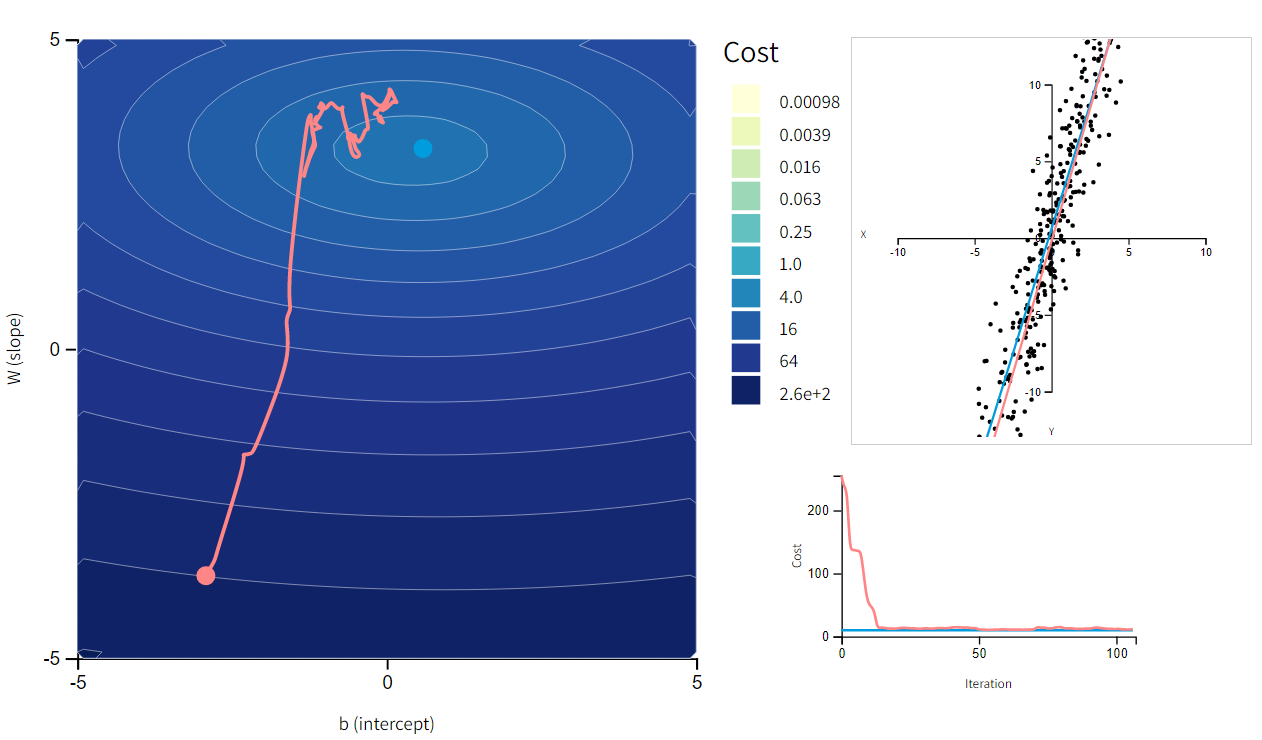
\includegraphics[width=7cm, height=4cm]{Figs/SGD.png}
%		    \caption{Stochastic Gradient Descent, From Hands-on Machine Learning}
%        \end{figure}
%    \end{itemize}
%\end{frame}
%
%\begin{frame}{Gradient Descent Algorithm Types}
%    \begin{itemize}
%        \item Stochastic Gradient Descent
%        \item Picks a random instance in the training set at every step
%        \begin{figure}
%            % \centering
%            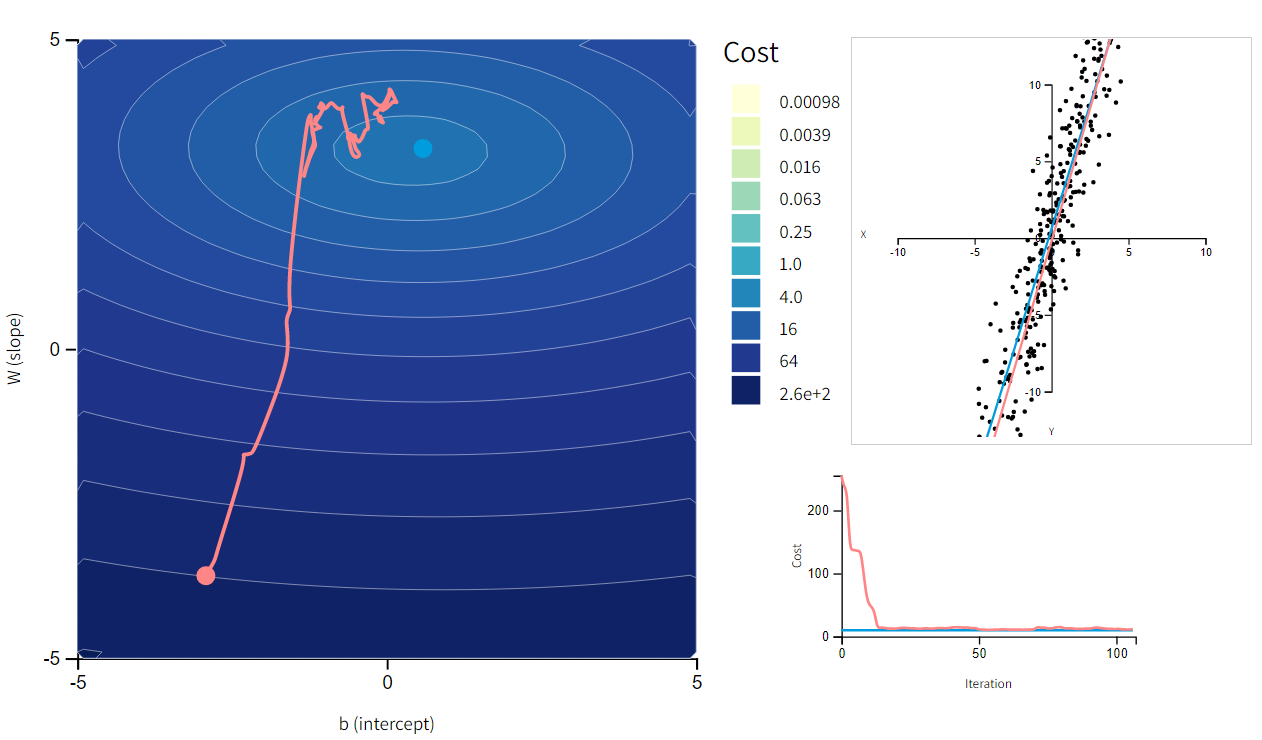
\includegraphics[width=7cm, height=4cm]{Figs/sgd.png}
%		    \caption{Stochastic Gradient Descent Cost Function}
%        \end{figure}
%    \end{itemize}
%\end{frame}


%%%%%%%%%%%%%%%%%%%%%%%%%%%%%%%%%%%%%%%%%%%%%%%%%%%%%%%%%%%%%%%%%%%%%%%%%%%%%%%%%%%%%%%%%%%%%%
%%%%%%%%%%%%%%%%%%%%%%%%%%%%%%%%%%%%%%%%%%%%%%%%%%%%%%%%%%%%%%%%%%%%%%%%%%%%%%%%%%%%%%%%%%%%%%
%%%%%%%%%%%%%%%%%%%%%%%%%%%%%%%%%%%%%%%%%%%%%%%%%%%%%%%%%%%%%%%%%%%%%%%%%%%%%%%%%%%%%%%%%%%%%%
%%%%%%%%%%%%%%%%%%%%%%%%%%%%%%%%%%%%%%%%%%%%%%%%%%%%%%%%%%%%%%%%%%%%%%%%%%%%%%%%%%%%%%%%%%%%%%
%%%%%%%%%%%%%%%%%%%%%%%%%%%%%%%%%%%%%%%%%%%%%%%%%%%%%%%%%%%%%%%%%%%%%%%%%%%%%%%%%%%%%%%%%%%%%%


\begin{frame}{Various GD types}
	\begin{itemize}
		\item So far you got familiar with gradient-based optimization.
		\item If $\bm{g} = \nabla_{\bm{\theta}} \mathcal{J}$, then we will update parameters with this simple rule:
		\[
		\bm{\theta} \gets \bm{\theta} - \eta\bm{g}
		\]
		% 	\item[]
		\item But there is one question here, how to compute $\bm{g}$?
		\item Based on how we calculate $\bm{g}$ we will have different types of gradient descent:
		\begin{itemize}
			\item Batch Gradient Descent
			\item Stochastic Gradient Descent
			\item Mini-Batch Gradient Descent
		\end{itemize}
	\end{itemize}
\end{frame}

\begin{frame}{Various GD types}
	\begin{block}{Recap:}
		Training cost function ($\mathcal{J}$) over a dataset usually is the average of loss function ($\mathcal{L}$) on entire training set, so for a dataset $\mathcal{D}=\{d_i\}_{i=1}^n$ we have:
		\[
		\mathcal{J}(\mathcal{D}) = \frac{1}{n} \sum_{i=1}^{n} \mathcal{L}(d_i; \bm{\theta})
		\]
		For example:
		\begin{equation*}
			H(p, q)=-\frac{1}{m} \sum_{i=1}^m\sum_{j=1}^{k} y_j^{(i)} \log (p(y_j^{(i)}))
		\end{equation*}
		\begin{equation*}
			\text{MSE}(y, \hat{y}) = \frac{1}{m}\sum_{i=1}^{m}(y_i-\hat{y}_i)^2
		\end{equation*}
		\begin{equation*}
			\text{MAE}(y, \hat{y}) = \frac{1}{m}\sum_{i=1}^{m}|(y_i-\hat{y}_i)|
		\end{equation*}
	\end{block}
\end{frame}

\begin{frame}{Various GD types: Batch Gradient Descent}
	\begin{itemize}
		\item In this type we use \tc{keywords}{entire training set} to calculate gradient.
		\begin{block}{Batch Gradient:}
			\[
			\bm{g} = \frac{1}{n}\sum_{i=1}^n \nabla_{\bm{\theta}} \mathcal{L}(d_i, \bm{\theta})
			\]
		\end{block}
		\item[]
		\item Using this method with very large training set:
		\begin{itemize}
			\item Your data can be too large to process in your memory.
			\item It requires a lot of processing to compute gradient for all samples.
		\end{itemize}
		\item Using exact gradient may lead us to local minima.
		\item Moving noisy may help us get out of this local minimas.
	\end{itemize}
\end{frame}

\begin{frame}{Various GD types: Batch Gradient Descent}
	\begin{figure}[H]
		\centering
		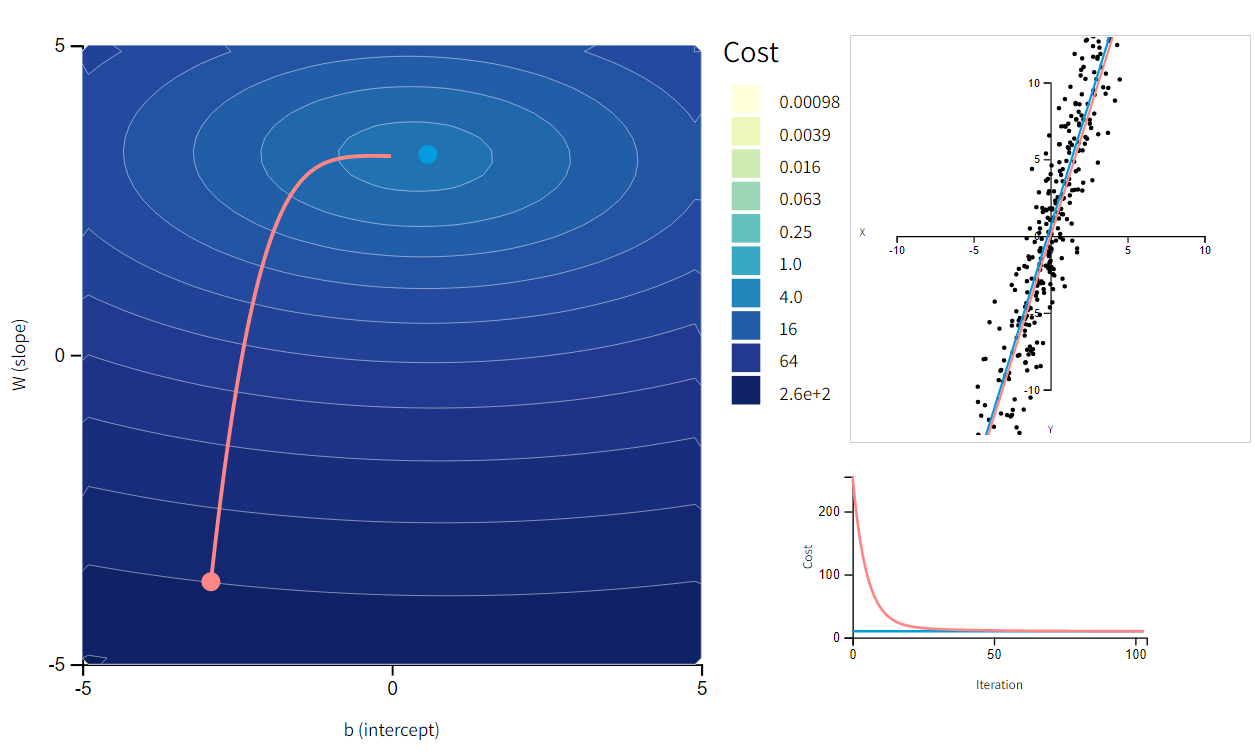
\includegraphics[width=0.8\textwidth]{Figs/bgd.png}
		\caption{Optimization of parameters using BGD. Movement is very smooth \cite{katanforoosh-kunin-opt}.}
	\end{figure} 
\end{frame}

\begin{frame}{Various GD types: Stochastic Gradient Descent}
	\begin{itemize}
		\item Instead of calculating exact gradient, we can estimate it using our data.
		\item This is exactly what SGD does, it estimates gradient using \tc{keywords}{only single data point}.
		\begin{block}{Stochastic Gradient:}
			\[
			\hat{\bm{g}} = \nabla_{\bm{\theta}} \mathcal{L}(d_i, \bm{\theta})
			\]
		\end{block}
		\item[]
		\item As we use an approximation of gradient, instead of gently decreasing, the cost function will bounce up and down and decrease only on average.
		\item This method is really computationally efficient cause we only need to calculate gradient for one point per iteration. 
	\end{itemize}
\end{frame}

\begin{frame}{Various GD types: Stochastic Gradient Descent}
	\begin{figure}[H]
		\centering
		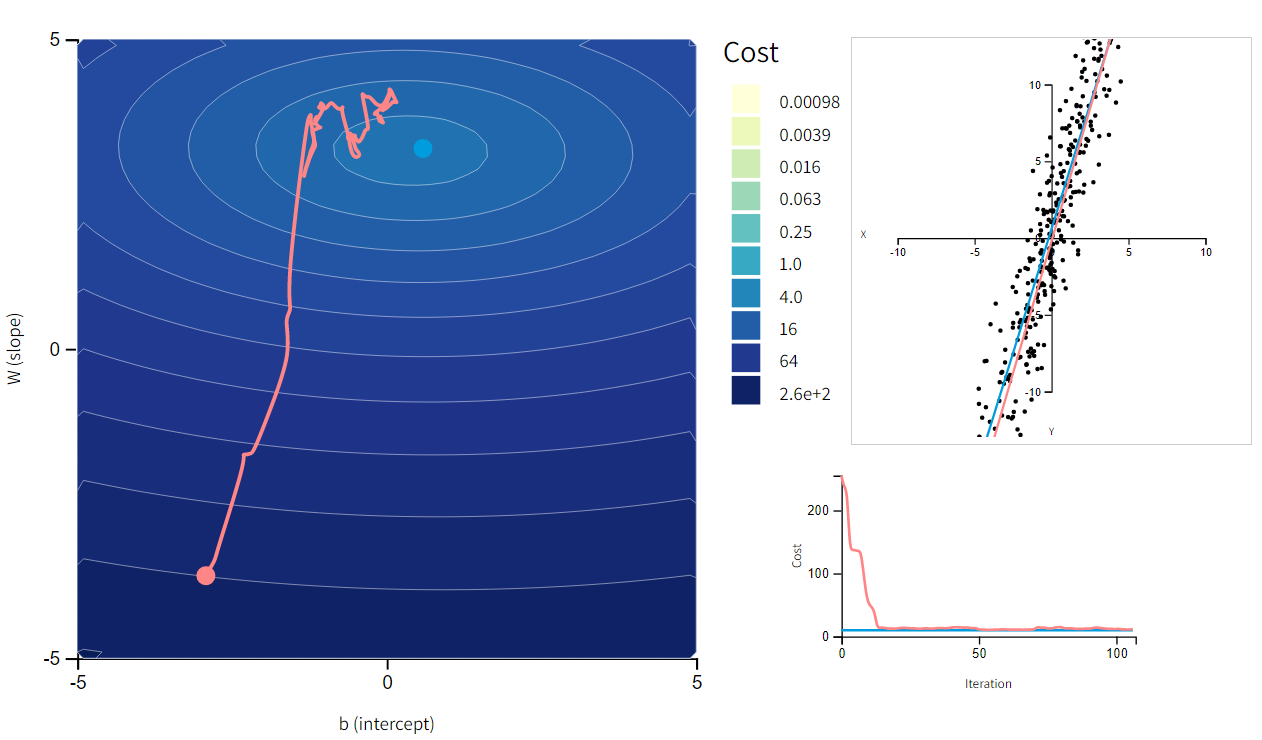
\includegraphics[width=0.8\textwidth]{Figs/sgd.png}
		\caption{Optimization of parameters using SGD. As we expect, the movement is not that smooth \cite{katanforoosh-kunin-opt}.}
	\end{figure} 
\end{frame}

\begin{frame}{Various GD types: Mini-Batch Gradient Descent}
	\begin{itemize}
		\item In this method we still use estimation idea But use \tc{keywords}{a batch of data} instead of one point.
		\begin{block}{Mini-Batch Gradient:}
			\[
			\hat{\bm{g}} = \frac{1}{|\mathcal{B}|} \sum_{d\in\mathcal{B}} \nabla_{\bm{\theta}} \mathcal{L}(d, \bm{\theta}), \quad \mathcal{B} \subset \mathcal{D}
			\]
		\end{block}
		\item[]
		\item This is a better estimation than SGD.
		\item With this way we can get a performance boost from hardware optimization, especially when using GPUs.
		\item Batch size ($|\mathcal{B}|$) is a hyperparameter you need to tune.
	\end{itemize}
\end{frame}

\begin{frame}{Various GD types: Mini-Batch Gradient Descent}
	\begin{figure}[H]
		\centering
		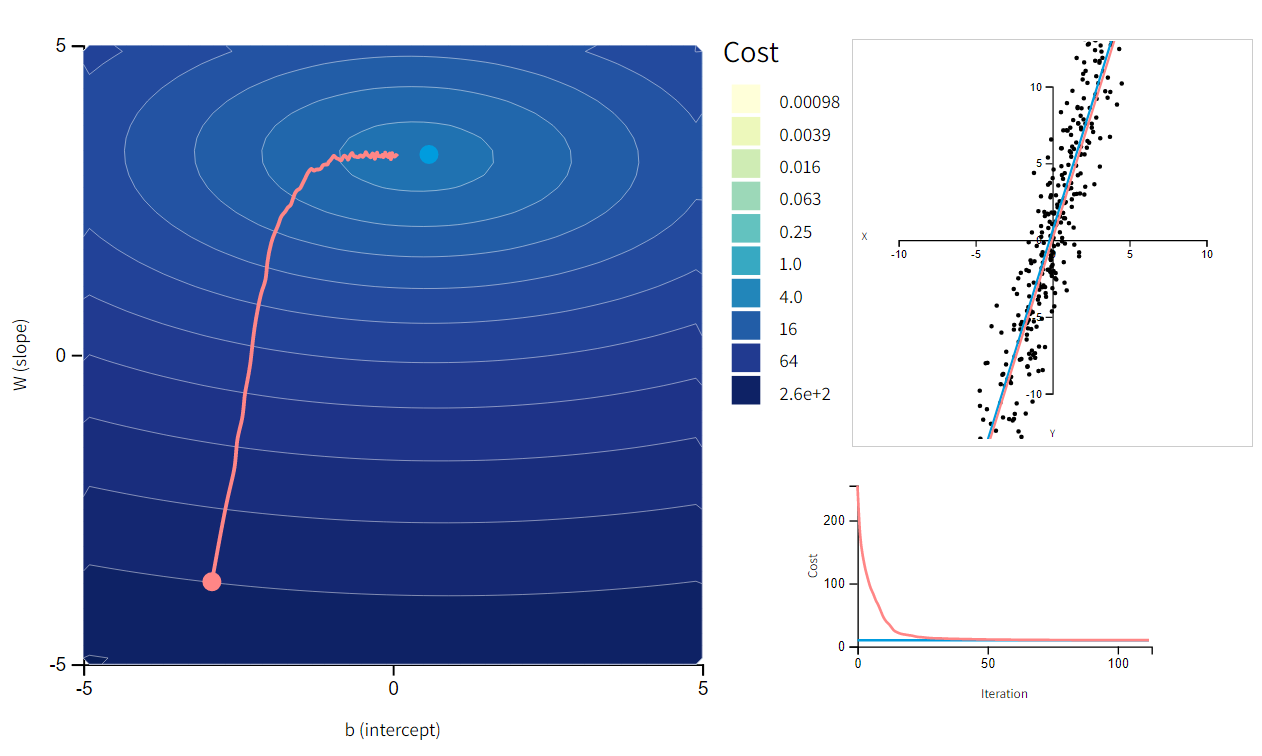
\includegraphics[width=0.8\textwidth]{Figs/mbgd.png}
		\caption{Optimization of parameters using MBGD. The movement is much smother than SGD and behave like BGD \cite{katanforoosh-kunin-opt}.}
	\end{figure} 
\end{frame}

\begin{frame}{Various GD types}
	\begin{itemize}
		\item Now that we know what a batch is, we can define epoch and iteration:
		\begin{itemize}
			\item One \tc{keywords}{Epoch} is when an entire dataset is passed forward and backward through the network only once.
			\item One \tc{keywords}{Iteration} is when a batch is passed forward and backward through the network. 
		\end{itemize}
		
		\begin{figure}[H]
			\centering
			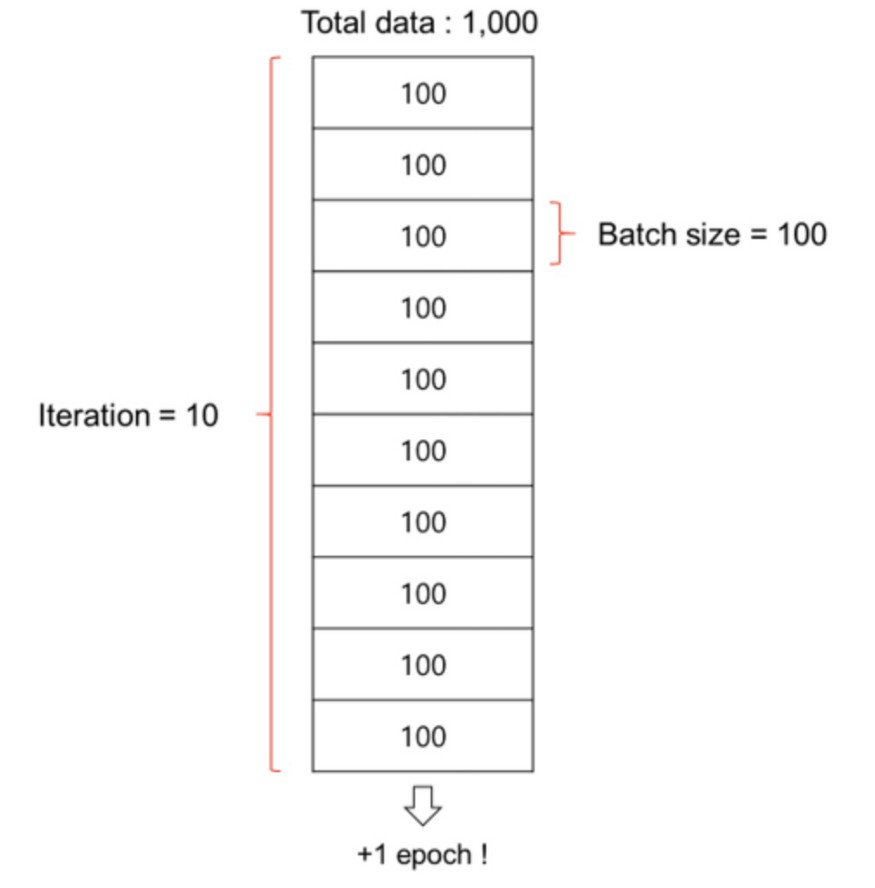
\includegraphics[width=0.4\textwidth]{Figs/epoch-iteration.png}
			\caption{Epoch vs Iteration, \href{https://jerryan.medium.com/batch-size-a15958708a6}{source}.}
		\end{figure} 
	\end{itemize}
\end{frame}

\begin{frame}{Various GD types}
	\begin{itemize}
		\item So we got familiar with different types of GD.
		\begin{itemize}
			\item[\color{darkgreen}$\checkmark$] Batch Gradient Descent (BGD)
			\item[\color{darkgreen}$\checkmark$] Stochastic Gradient Descent (SGD)
			\item[\color{darkgreen}$\checkmark$] Mini-Batch Gradient Descent (MBGD)
		\end{itemize}
		\item[]
		\item[]
		\item The most recommended one is MBGD, because it is computational efficient.
		\item Choosing the right batch size is important to ensure convergence of the cost function and parameter values, and to the generalization of your model.
	\end{itemize}
\end{frame}